\section{Introdução}\label{introduuxe7uxe3o}

Esta prática tem como objetivo criar um semáforo de carros e pedestres
usando a ferramenta SanUSB \cite{sanusb-mplabx:11} e microcontrolador
PIC18F4550 \cite{microchip-pic18f4550}, em que o pedestre pode solicitar
sua passagem e visualizar um display de 7 segmentos que mostra o tempo
que ele tem para fazer a passagem. Imagine que este semáforo está em uma
auto estrada de alta velocidade. Nesse cenário o sinal para os carros
está sempre verde e para os pedestres está sempre vermelho. Quando um
pedestre solicita a passagem através de um botão, o sinal para os carros
sai do vermelho para o amarelo, logo em seguida para o vermelho,
enquanto isso o sinal dos pedestres vai para o verde e um par de
displays de 7 segmentos mostra o tempo que o pedestre tem para
atravessar a auto estrada antes que o sinal fique verde para os carros
novamente.

\section{Material Necessário}\label{material-necessuxe1rio}

\begin{itemize}
\itemsep1pt\parskip0pt\parsep0pt
\item
  5 LEDs
\item
  7 Resistores $390 \Omega$
\item
  2 Displays de 7 segmentos
\item
  1 Cabo USB
\item
  1 Placa SanUSB
\item
  1 Protoboard
\end{itemize}

A programação é feita através da MPLAB-X IDE \cite{mplabx-ide} e a
gravação é feita com o Gravador SanUSB \cite{gravador-sanusb}.

\section{Iteração 1 - Semáforo
simples}\label{iterauxe7uxe3o-1---semuxe1foro-simples}

Inicialmente faremos um semáforo simples apenas dos carros, como mostra
a Figura \ref{fig:semaforo-1}.

\begin{figure}[h]
    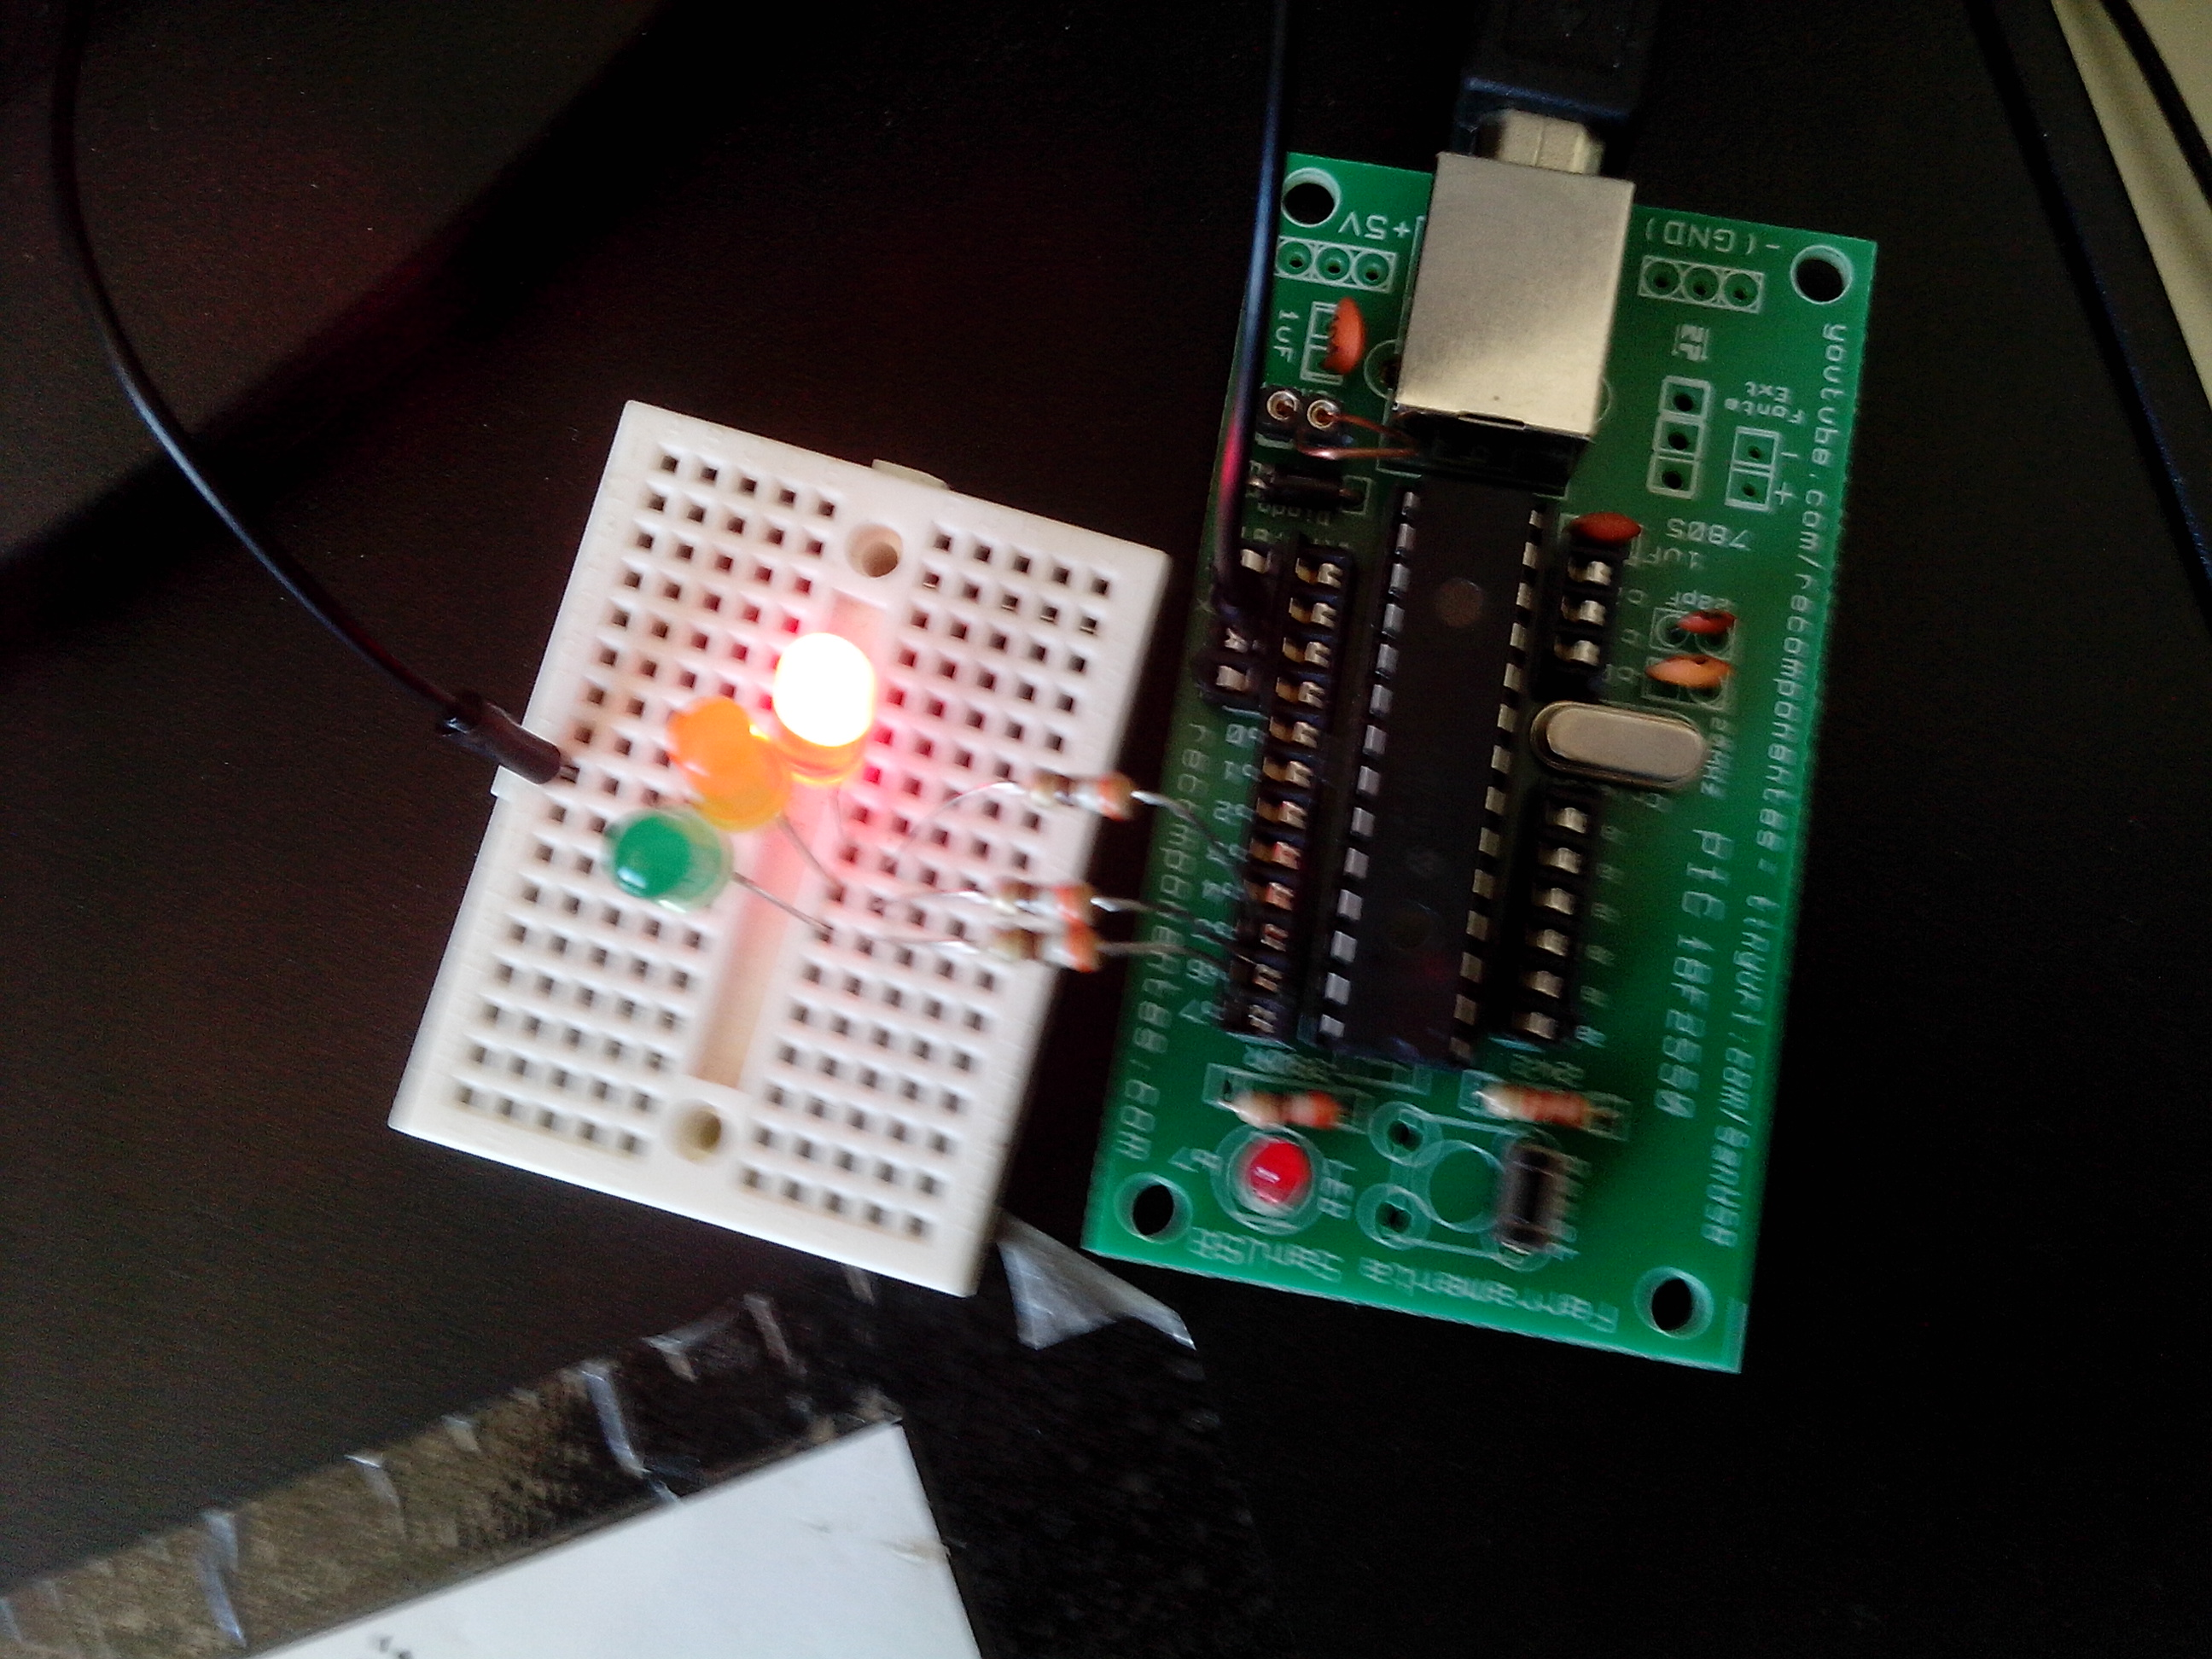
\includegraphics[scale=0.5]{img/semaforo-1.jpg}
    \caption{Semáforo Simples de Carros} \label{fig:semaforo-1}
\end{figure}

Código Fonte da iteração 1 no Apêndice \ref{source:iteracao-1}.

\section{Iteração 2 - Semáforo simples para carros e
pedestres}\label{iterauxe7uxe3o-2---semuxe1foro-simples-para-carros-e-pedestres}

Em seguida faremos um semáforo tanto para os carros quanto para os
pedestres. O semáforo deve estar sempre verde para os carros e vermelho
para os pedestres. Ao acionar um botão o semáforo entra num processo em
que o sinal alterna por um tempo.

\begin{figure}[H]
    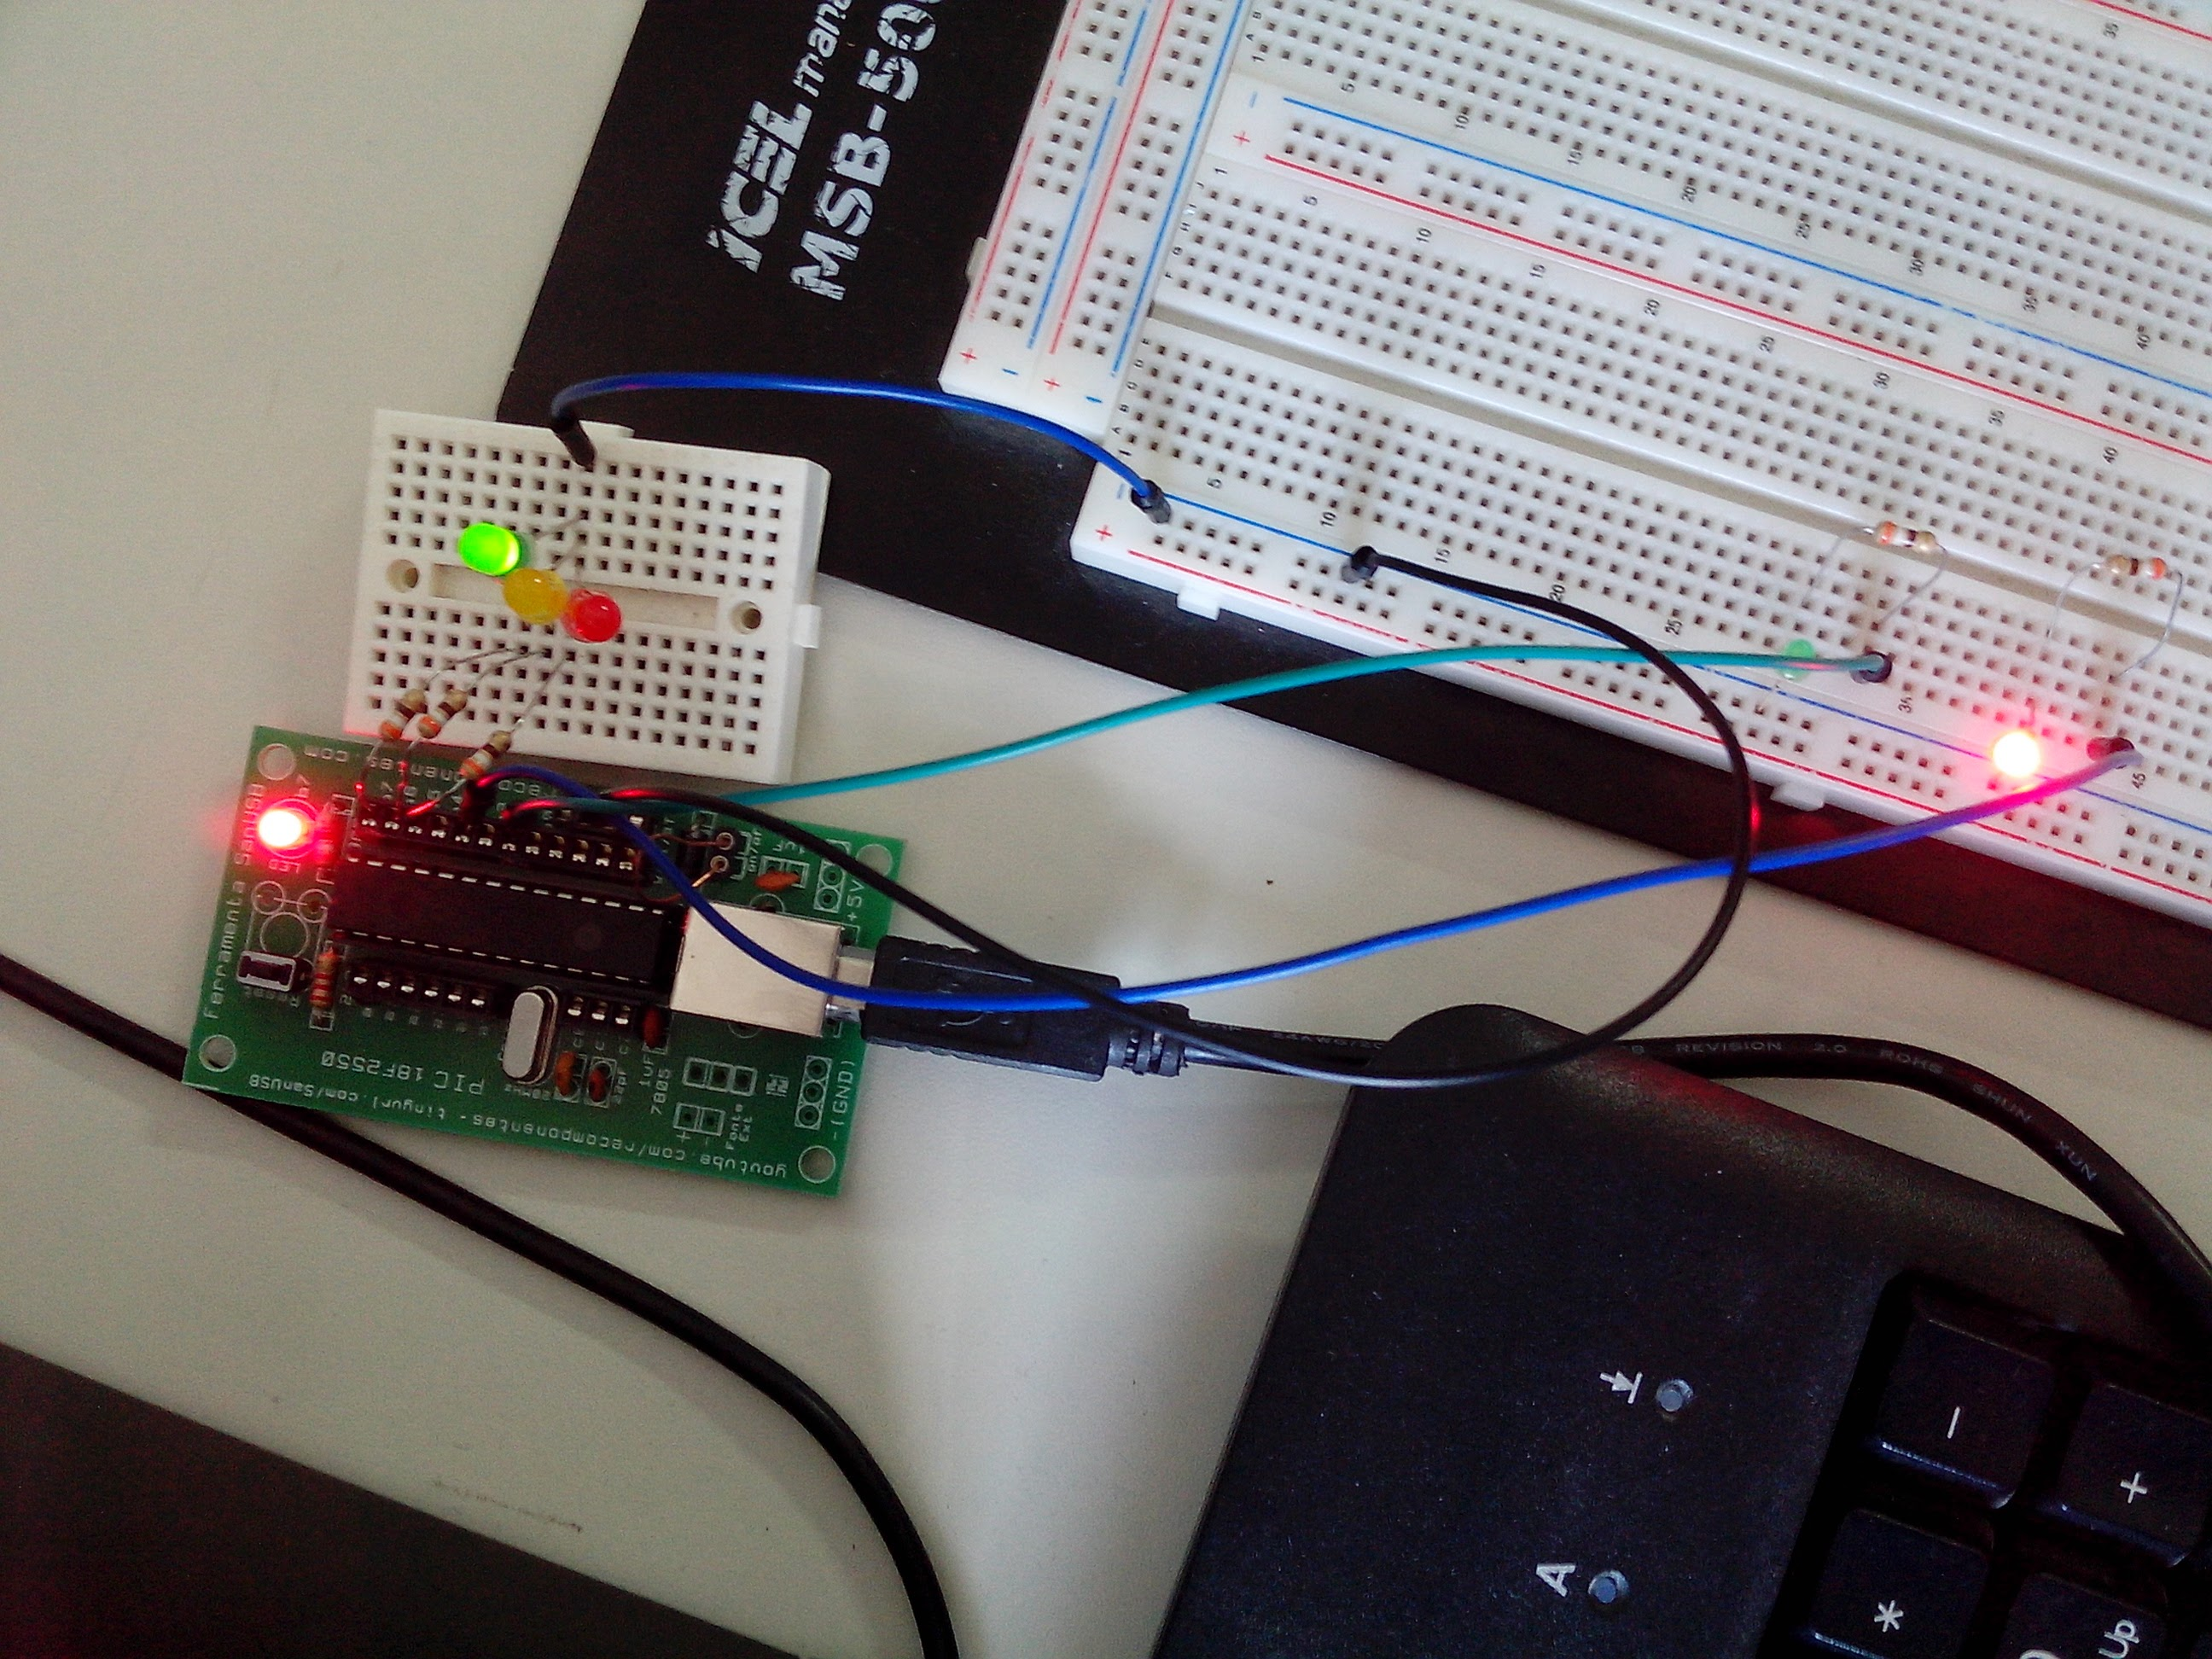
\includegraphics[scale=0.5]{img/semaforo-2.jpg}
    \caption{Semáforo simples para carros e pedestres}
\end{figure}

Código Fonte da iteração 2 no Apêndice \ref{source:iteracao-2}.

\section{Iteração 3 - Display de 7 segmentos com contagem
regressiva}\label{iterauxe7uxe3o-3---display-de-7-segmentos-com-contagem-regressiva}

Com o semáforo produzido é preciso usar um display de 7 segmentos que
irá mostrar a contagem regressiva para que o sinal verde do pedestre vá
para vermelho. Mas antes é preciso fazer apenas que o display conte de
zero a nove indefinidamente.

\begin{figure}[H]
    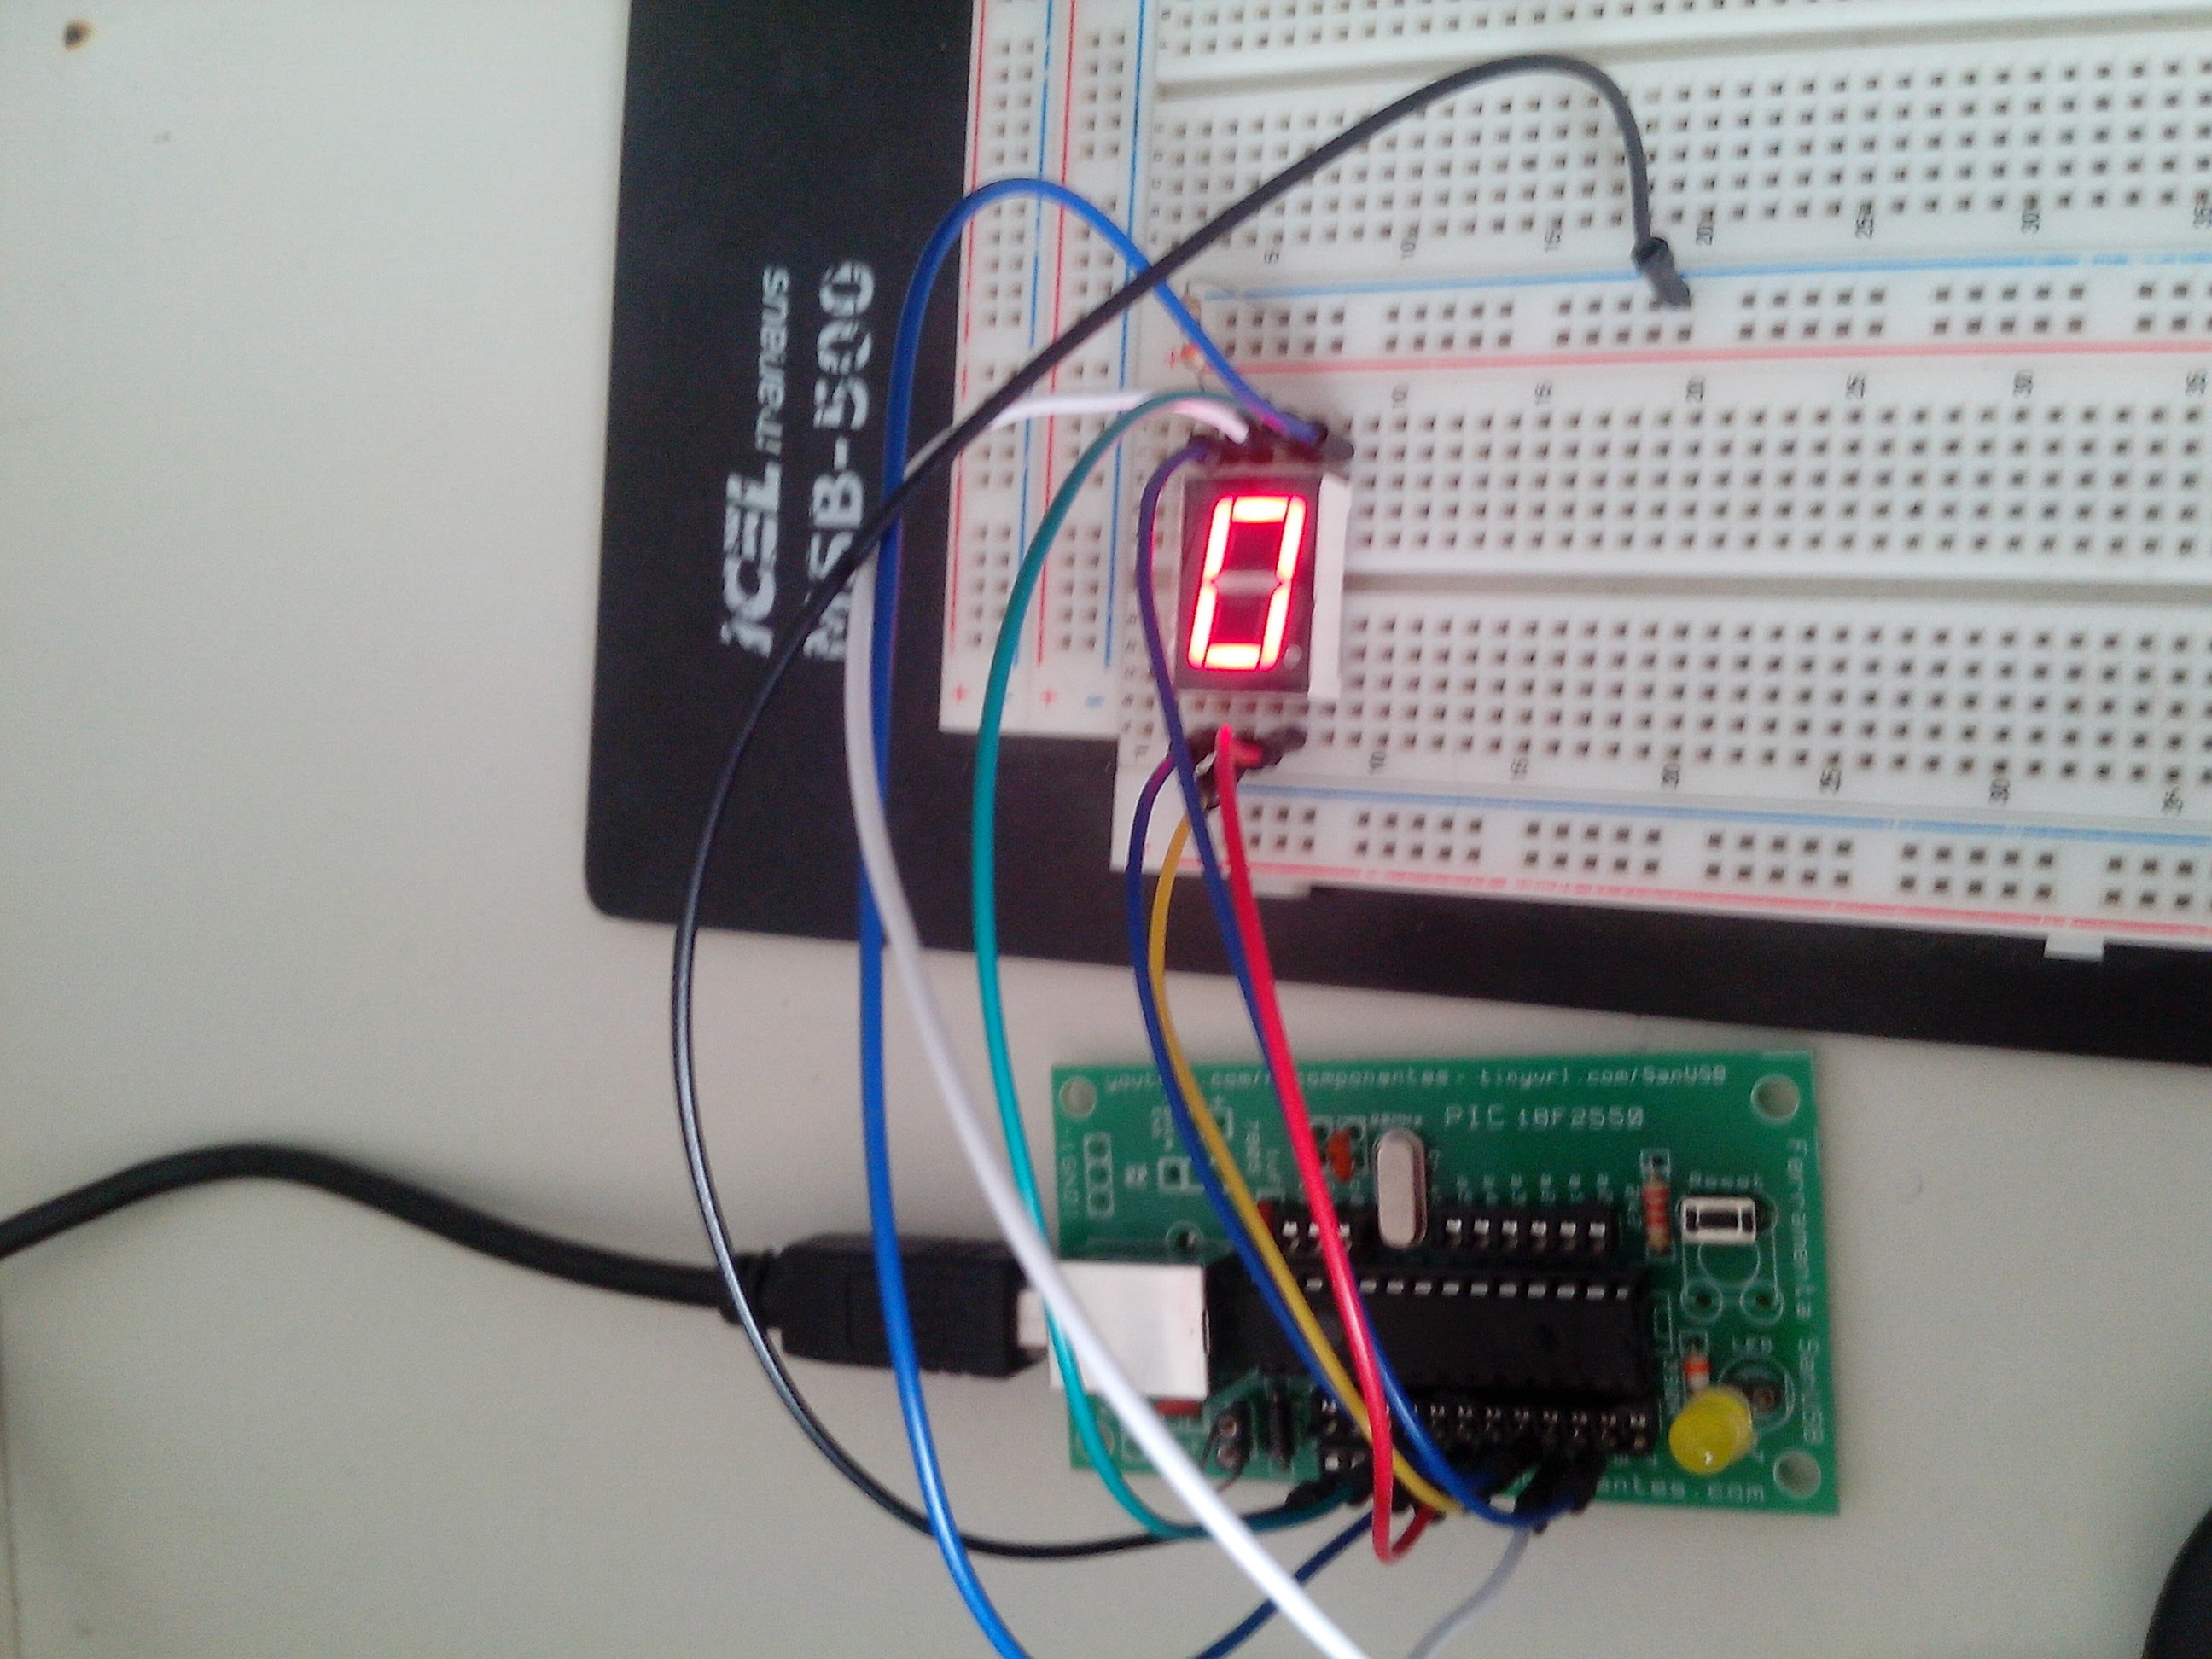
\includegraphics[scale=0.5]{img/display-7seg-1.jpg}
    \caption{Display de 7 segmentos com contagem regressiva} \label{fig:display-7seg-1}
\end{figure}

Código Fonte da iteração 3 no Apêndice \ref{source:iteracao-3}.

\section{Iteração 4 - 2 displays de 7 segmentos
multiplexados}\label{iterauxe7uxe3o-4---2-displays-de-7-segmentos-multiplexados}

Como visto na Figura \ref{fig:display-7seg-1}, um único display de 7
segmentos ocupa 7 pinos e um GND da placa. Sendo assim para conseguir
usar 2 displays seriam necessários 14 pinos, o que torna o projeto mais
complexo e caro.

Para resolver esse problema basta aplicar a multiplexação, fazendo com
que os pinos sejam controlados por pinos chamados pinos de controle.
Para ligar 2 displays colocamos os segmentos em curto e trocar o GND por
dois pinos na placa. O estado do pino é alternado em espaços curtos de
tempo de forma que dê a impressão que os displays estão acesos ao mesmo
tempo.

Veja o circuito montado na Figura \ref{fig:display-7seg-2}.

\begin{figure}[H]
    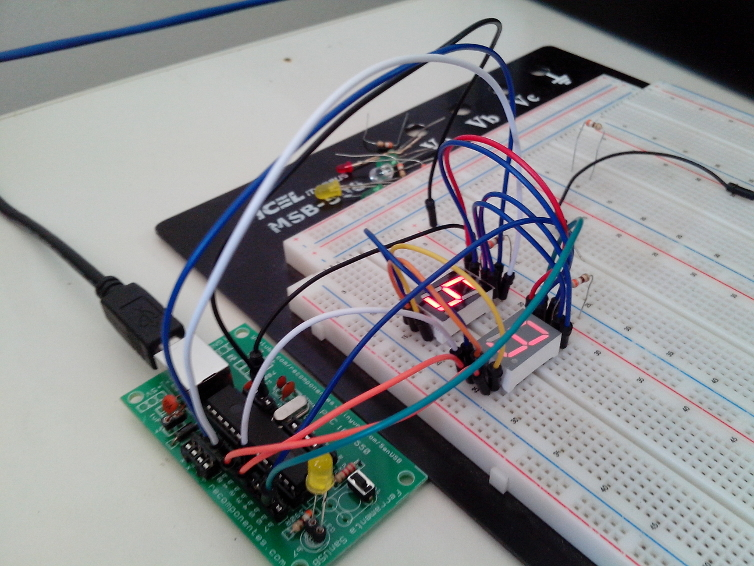
\includegraphics[scale=0.5]{img/display-7seg-2.jpg}
    \caption{Multiplexação de 2 Displays de 7 segmentos} \label{fig:display-7seg-2}
\end{figure}

Código Fonte da iteração 4 no Apêndice \ref{source:iteracao-4}.

\section{Iteração 5 - Semáforo para carros e pedestres com contagem
regressiva}\label{iterauxe7uxe3o-5---semuxe1foro-para-carros-e-pedestres-com-contagem-regressiva}

A partir do conteúdo já visto é possível criar um semáforo para carros e
pedestres com contagem regressiva.

O circuito completo pode ser visto na Figura \ref{semaforo-3}.

\begin{figure}[H]
    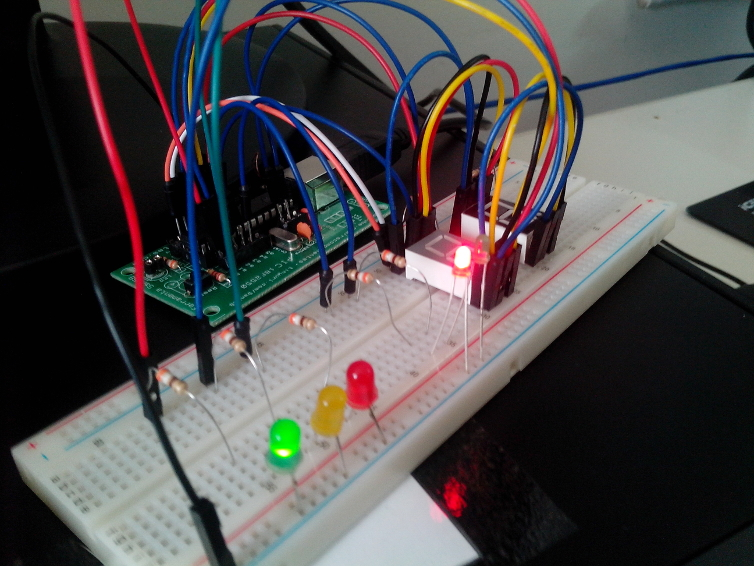
\includegraphics[scale=0.5]{img/semaforo-3.jpg}
    \caption{Semáforo para carros e pedestres com contagem regressiva} \label{semaforo-3}
\end{figure}

Código Fonte da iteração 5 no Apêndice \ref{source:iteracao-5}.
